% --- Template for thesis / report with tktltiki2 class ---
% 
% last updated 2013/02/15 for tkltiki2 v1.02

\documentclass[english]{tktltiki2}

% tktltiki2 automatically loads babel, so you can simply
% give the language parameter (e.g. finnish, swedish, english, british) as
% a parameter for the class: \documentclass[finnish]{tktltiki2}.
% The information on title and abstract is generated automatically depending on
% the language, see below if you need to change any of these manually.
% 
% Class options:
% - grading                 -- Print labels for grading information on the front page.
% - disablelastpagecounter  -- Disables the automatic generation of page number information
%                              in the abstract. See also \numberofpagesinformation{} command below.
%
% The class also respects the following options of article class:
%   10pt, 11pt, 12pt, final, draft, oneside, twoside,
%   openright, openany, onecolumn, twocolumn, leqno, fleqn
%
% The default font size is 11pt. The paper size used is A4, other sizes are not supported.
%
% rubber: module pdftex

% --- General packages ---

\usepackage[utf8]{inputenc}
\usepackage[T1]{fontenc}
\usepackage{lmodern}
\usepackage{microtype}
\usepackage{amsfonts,amsmath,amssymb,amsthm,booktabs,color,enumitem,graphicx}
\usepackage[pdftex,hidelinks]{hyperref}

% Automatically set the PDF metadata fields
\makeatletter
\AtBeginDocument{\hypersetup{pdftitle = {\@title}, pdfauthor = {\@author}}}
\makeatother

% --- Language-related settings ---
%
% these should be modified according to your language

% babelbib for non-english bibliography using bibtex
\usepackage[fixlanguage]{babelbib}

% add bibliography to the table of contents
\usepackage[nottoc]{tocbibind}

% --- Theorem environment definitions ---

\newtheorem{thm}{Theorem}
\newtheorem{lem}[thm]{Lemma}
\newtheorem{cor}[thm]{Corollary}

\theoremstyle{definition}
\newtheorem{definition}[thm]{Definition}

\theoremstyle{remark}
\newtheorem*{remark}{Remark}


% --- tktltiki2 options ---
%
% The following commands define the information used to generate title and
% abstract pages. The following entries should be always specified:

\title{Extending the “Development Pipeline” Towards Continuous Deployment and Continuous Experimentation: A Case Study in the B2B Domain}
\author{Olli Rissanen}
\date{\today}
\level{Master's thesis}
\abstract{Currently more and more software companies are moving to lean practices, which often include shorter delivery cycles and thus shorter feedback loops. However, to achieve continuous customer feedback and to eliminate work that doesn't generate value, even shorter cycles are required. In continuous deployment the software functionality is deployed continuously at customer environment. This process includes both automated builds and automated testing, but also automated deployment. Automating the whole process minimizes the time required for implementing new features in software, and allows for faster customer feedback. However, adopting continuous deployment doesn't necessarily mean that more value is created for the customer. While continuous deployment attempts to deliver an idea to users as fast as possible, continuous experimentation instead attempts to validate that it is, in fact, a good idea. In a state of continuous experimentation, the entire R\&D process is guided by controlled experiments and feedback. In it's core continuous experimentation consists of a design-execute-analyse loop, where hypotheses are selected based on business goals and strategies, experiments are executed with partial implementations and data collection tools and finally the results are analyzed to validate the hypothesis. In this paper we're ..}

% The following can be used to specify keywords and classification of the paper:

\keywords{Continuous delivery, Continuous experimentation, Development pipeline}

% classification according to ACM Computing Classification System (http://www.acm.org/about/class/)
% This is probably mostly relevant for computer scientists
% uncomment the following; contents of \classification will be printed under the abstract with a title
% "ACM Computing Classification System (CCS):"
% \classification{}

% If the automatic page number counting is not working as desired in your case,
% uncomment the following to manually set the number of pages displayed in the abstract page:
%
% \numberofpagesinformation{16 pages + 10 appendix pages}
%
% If you are not a computer scientist, you will want to uncomment the following by hand and specify
% your department, faculty and subject by hand:
%
\faculty{Faculty of Science}
\department{Department of Computer Science}
\subject{Computer Science}
%
% If you are not from the University of Helsinki, then you will most likely want to set these also:
%
\university{University of Helsinki}
% \universitylong{HELSINGIN YLIOPISTO --- HELSINGFORS UNIVERSITET --- UNIVERSITY OF HELSINKI} % displayed on the top of the abstract page
\city{Helsinki}
%


\begin{document}

% --- Front matter ---

\frontmatter      % roman page numbering for front matter

\maketitle        % title page
\makeabstract     % abstract page

\tableofcontents  % table of contents

% --- Main matter ---

\newpage

It’s hard to argue that Tiger Woods is pretty darn good at what he does. But even he is not perfect. Imagine if
he were allowed to hit four balls each time and then choose the shot that worked the best. Scary good.
-- Michael Egan, Sr. Director, Content Solutions, Yahoo (Egan, 2007)

\mainmatter       % clear page, start arabic page numbering



%case study
% Relate the theory to a practical situation; for example, apply the ideas 
%and knowledge discussed in the coursework to the practical situation 
%at hand in the case study. 
 
% Identify the problems 
% Select the major problems in the case 
% Suggest solutions to these major problems 
% Recommend the best solution to be implemented 
% Detail how this solution should be implemented

\section{Introduction}
-GOAL OF THE THESIS
-motivation
-research question
-approach

>analyze state of the practice
>specify problem and goals 
>analyze state of the art
>state hypotheses
>derive solution idea

\section{Related work}
-continuous delivery
-continuous experimentation
-state of the art practices
    -short summary

\subsection{Continuous delivery}
Continuous deployment is an extension to continuous integration, where the software functionality is deployed frequently at customer environment. While continuous integration defines a process where the work is automatically built, tested and frequently integrated to mainline \cite{fowler2006continuous}, often multiple times a day, continuous deployment adds automated acceptance testing and deployment. The purpose of continuous deployment is that as the deployment process is completely automated, it reduces human error, documents required for the build and increases confidence that the build works \cite{cdbook}. %Explain pipeline here

An important part of continuous deployment is the deployment pipeline, which is an automated implementation of an application's build, deploy, test and release process \cite{cdbook}. A deployment pipeline can be loosely defined as a consecutively executed set of validations that a software has to pass such before it can be released. Common components of the deployment pipeline are a version control system and an automated test suite.

In an agile process software release is done in periodic intervals \cite{cockburn2002agile}. Compared to waterfall model it introduces multiple releases throughout the development. Continuous deployment, on the other hand, attemps to keep the software ready for release at all times during development process \cite{cdbook}. Instead of stopping the development process and creating a build as in an agile process, the software is continuously deployed to customer environment. This doesn't mean that the development cycles in continuous deployment are shorter, but that the development is done in a way that makes the software always ready for release.

It should also be made clear that continuous delivery differs from continous deployment. Refer to Fig. \ref{fig1} for a visual representation of differences in continuous integration, delivery and deployment. Both include automated deployment to a staging environment. Continuous deployment includes deployment to a production environment, while in continuous delivery the deployment to a production environment is done manually. The purpose of continuous delivery is to prove that every build is proven deployable \cite{cdbook}. While it necessarily doesn't mean that teams release often, keeping the software in a state where a release can be made instantly is often seen beneficial.

\subsection{Experimentation}
An experiment is essentially a procedure to confirm the validity of a hypothesis. In software engineering context, experiments attempt to answer questions such as which features are necessary for a product to succeed, what should be done next and which customer opinions should be listened to. According to Jan Bosch, "The faster the organization learns about the customer and the real world operation of the system, the more value it will provide" \cite{bosch2012building}. Most organizations have many ideas, but the return-on-investment for many may be unclear and the evaluation itself may be expensive \cite{kohavi2007practical}. I

In Lean startup methodology \cite{ries2011lean} experiments consist of Build-Measure-Learn cycles, and are tightly connected to visions and the business strategy. The purpose of a Build-Measure-Learn cycle is to turn ideas into products, measure how customers respond to the product and then to either pivot or persevere the chosen strategy. The cycle starts with forming a hypothesis and building a minimum viable product (MVP) with tools for data collection. Once the MVP has been created, the data is analyzed and measured in order to validate the hypothesis. To persevere with a chosen strategy means that the experiment proved the hypothesis correct, and the full product or feature can is implemented. However, if the experiment proved the hypothesis wrong, the strategy is changed based on the implications of a false hypothesis.

Jan Bosch has widely studied continuous experimentation, or innovation experiment systems, as a basis for development. The primary issue he found is that "experimentation in online software is often limited to optimizing narrow aspects of the front-end of the website through A/B testing and inconnected, software-intensive systems experimentation, if applied at all, is ad-hoc and not systematically applied" \cite{bosch2012building}. The author realized that for different development stages, different techniques to implement experiments and collect customer feedback exist. Bosch also introduces a case study in which a company, Intuit, adopted continuous experimentation and has increased both the performance of the product and customer satisfaction.

Fig. \ref{fig4} introduces different stages and scopes for experimentation. For each stage and scope combination, an example technique to collect product performance data is shown. As startups often start new products and older companies instead develop new features, experiments must be applied in the correct context. Bosch states that for a new product deployment, putting a minimal viable product as rapidly as possible in the hands of customers is essential \cite{bosch2012building}. After the customers can use the product, it is often not yet monetizable but is still of value to the customer. Finally, the product is commercially deployed and collecting feedback is required to direct R\&D investments to most valuable features.
\begin{figure}[H]
	\centering
	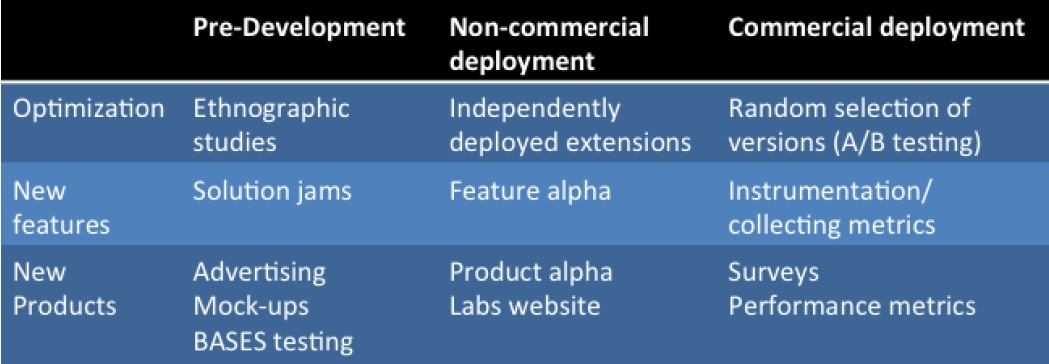
\includegraphics[width=3.5in]{bosch.jpg}
	\caption{Scopes for experimentation\cite{bosch2012building}.}
	\label{fig4}
\end{figure}

\subsection{Continuous experimentation}
Continuous deployment attempts to deliver an idea to users as fast as possible. Continuous experimentation instead attempts to validate that it is, in fact, a good idea. In continuous experimentation the organisation runs controlled experiments to guide the R\&D process. The development cycle in continuous experimentation resembles the build-measure-learn cycle of lean startup \cite{ries2011lean}. The process in continuos experimentation is to first form a hypothesis based on a business goals and customer "pains" \cite{bosch2012building}. After the hypothesis has been formed, quantitative metrics to measure the hypothesis must be decided. After this a minimum viable product can be developed and deployed, while collecting the required data. Finally, the data is analyzed to attempt to validate the hypothesis.

As the experiments are run in a regular fashion, it integratign experiments to the deployment pipeline should be considered. This requires changing the development process in such fashion that functionality is developed based on some actual data. The components required to support continuous experimentation include tools to assign users to treatment and control groups, tools for data logging and storing, and analytics tool for conducting statistical analyses.

\subsection{State of the art}

\subsection{State of the practice}	
%Introduce steeri
Steeri is a mid-sized company of 80 employees, focusing in managing and improving customer data usage. This includes CRM systems, business intelligence solutions, customer dialog and data integration. Steeri has created Customer data management (CDM) and Customer dialog (Dialog) products, which are developed by two different teams. 

These two teams develop in an agile manner, but the continuous integration process \cite{fowler2006continuous} and short feedback cycles aren't achieved yet. 

The development isn't at all distributed, and no external party affects the development process. 

\cite{olsson2012climbing}

-current state at steeri
    -short summary

Be sure to specify as much of the industrial context as possible. In particular,
clearly define the entities, attributes, and measures that are capturing the contextual information.


\section{Needs, problems and challenges}

\subsection{Problems}
-Collecting feedback in a B2B environment
-The time between the idea and implementation is too long
-Time dimension. If an impact is done right now, when will the effects be visible?
-Conventions for production deployment. The whole pipe between the idea and implementation isn't yet completely perceived. Some parts are visible, but the entirety is still unclear.
-How do we validate whether a feature is succesful or not? In B2C this is usually done by observing shifts in sales, but in our product there's no such thing.
-Possibly things we can analyze are user experience, but is it enough?

\section{Research method}

Exploratory case study: Finding out what is happening, seeking new insights and generating ideas and hypotheses for new research.

Case study structure: 

1. Case study design: objectives are defined and 
the case study is planned. 
2. Preparation for data collection: procedures and 
protocols for data collection are defined. 
3. Collecting evidence: execution with data 
collection on the studied case. 
4. Analysis of collected data 
5. Reporting 

Proposal for solution


\section{Hypothesis}
\section{Methodology}
Adopt the solution
Implement & test

\section{Results}
\section{Analysis}
\section{Conclusion}


% --- References ---
%
% bibtex is used to generate the bibliography. The babplain style
% will generate numeric references (e.g. [1]) appropriate for theoretical
% computer science. If you need alphanumeric references (e.g [Tur90]), use
%
% \bibliographystyle{babalpha-lf}
%
% instead.

\bibliographystyle{babplain-lf}
\bibliography{gradu}


% --- Appendices ---

% uncomment the following

% \newpage
% \appendix
% 
% \section{Example appendix}

\end{document}
